% This is "sig-alternate.tex" V2.0 May 2012
% This file should be compiled with V2.5 of "sig-alternate.cls" May 2012
%
% This example file demonstrates the use of the 'sig-alternate.cls'
% V2.5 LaTeX2e document class file. It is for those submitting
% articles to ACM Conference Proceedings WHO DO NOT WISH TO
% STRICTLY ADHERE TO THE SIGS (PUBS-BOARD-ENDORSED) STYLE.
% The 'sig-alternate.cls' file will produce a similar-looking,
% albeit, 'tighter' paper resulting in, invariably, fewer pages.
%
% ----------------------------------------------------------------------------------------------------------------
% This .tex file (and associated .cls V2.5) produces:
%       1) The Permission Statement
%       2) The Conference (location) Info information
%       3) The Copyright Line with ACM data
%       4) NO page numbers
%
% as against the acm_proc_article-sp.cls file which
% DOES NOT produce 1) thru' 3) above.
%
% Using 'sig-alternate.cls' you have control, however, from within
% the source .tex file, over both the CopyrightYear
% (defaulted to 200X) and the ACM Copyright Data
% (defaulted to X-XXXXX-XX-X/XX/XX).
% e.g.
% \CopyrightYear{2007} will cause 2007 to appear in the copyright line.
% \crdata{0-12345-67-8/90/12} will cause 0-12345-67-8/90/12 to appear in the copyright line.
%
% ---------------------------------------------------------------------------------------------------------------
% This .tex source is an example which *does* use
% the .bib file (from which the .bbl file % is produced).
% REMEMBER HOWEVER: After having produced the .bbl file,
% and prior to final submission, you *NEED* to 'insert'
% your .bbl file into your source .tex file so as to provide
% ONE 'self-contained' source file.
%
% ================= IF YOU HAVE QUESTIONS =======================
% Questions regarding the SIGS styles, SIGS policies and
% procedures, Conferences etc. should be sent to
% Adrienne Griscti (griscti@acm.org)
%
% Technical questions _only_ to
% Gerald Murray (murray@hq.acm.org)
% ===============================================================
%
% For tracking purposes - this is V2.0 - May 2012

%\documentclass[10pt, conference, compsocconf]{IEEEtran}
%\documentclass[10pt,conference]{IEEEtran} 
%\documentclass{sig-alternate}
\documentclass[sigconf,review, anonymous]{acmart}
\acmConference[ICSE 2018]{40th International Conference on Software Engineering}{May 27--June 3, 2018}{Gothenburg, Sweden}
\acmYear{2018}

\usepackage{url}
\usepackage{balance}
\usepackage{hyperref}
\usepackage{graphicx}
\usepackage{xspace}
\usepackage{color}
\usepackage{pifont}
\usepackage{xcolor,colortbl}

\usepackage[framemethod=TikZ]{mdframed}
\usepackage{lipsum}
\mdfdefinestyle{ExampleFrame}{
	linecolor=black,
	linewidth=1pt,
	frametitlerule=true,
	frametitlebackgroundcolor=gray!20,
	innertopmargin=\topskip,
	roundcorner=5pt
}


%\newenvironment{widequotation}{\list{}{\listparindent 1.5em \itemindent\listparindent
%		\rightmargin 0pt \parsep 0pt plus 1pt}\item\relax}
%{\endlist}
%\def\signed#1{{\leavevmode\unskip\nobreak\hfil\penalty50\hskip2em
%		\hbox{}\nobreak\hfil\raise-1pt\hbox{#1}%
%		\parfillskip=0pt \finalhyphendemerits=0 \endgraf}}
%\newsavebox\mybox
%\newenvironment{aquote}[1]
%	{\savebox\mybox{(#1)}\begin{widequotation}\itshape``\ignorespaces}
%	{\unskip"\signed{\usebox\mybox}\end{widequotation}}


\sloppy
\newcommand {\pl}[1]{[{\bf \textcolor{green} \underline{Patricia}}: {\bf #1}]}
\newcommand {\pat}[1]{[{\bf \underline{Patrizio}}: {\bf #1}]}
\newcommand {\rog}[1]{[{\bf \underline{Rogardt}}: {\bf #1}]}
\newcommand{\todo}[1]{\textcolor{blue}{\ding{46}~{\sf todo}~#1}}

%\newcommand{\definition}[2]{\noindent \textbf{\emph{Definition #1}} (#2)}
\newcommand{\ttransition}[2]{\stackrel{#1}{\longrightarrow^{#2}}}
\newcommand{\ntransition}[1]{\longrightarrow^{#1}}
\newcommand{\transition}[1]{\stackrel{#1}{\rightarrow}}
\newcommand{\Transition}[1]{\stackrel{#1}{\Rightarrow}}
\newcommand{\freccia}[1]{\mathop{\stackrel{#1} {\longrightarrow}} }
\newcommand{\ug}[1]{\mathop{=}\limits^{#1}_{}}
\newcommand{\barra}[1]{\overline{#1}}
\newcommand{\eqdef}{\stackrel{def}{=}}


\newcommand{\footlabel}[2]{%
    \addtocounter{footnote}{1}%
    \footnotetext[\thefootnote]{%
        \addtocounter{footnote}{-1}%
        \refstepcounter{footnote}\label{#1}%
        {\footnotesize #2}%
    }%
    $^{\ref{#1}}$%
}

\newcommand{\footref}[1]{%
    $^{\ref{#1}}$%
}

\usepackage{listings}

% colors
\definecolor{mygreen}{rgb}{0,0.6,0}
\definecolor{mygray}{rgb}{0.5,0.5,0.5}
\definecolor{mymauve}{rgb}{0.58,0,0.82}
\definecolor{light-gray}{gray}{0.85}

% listing settings
\lstset{ %
  backgroundcolor=\color{white},   % choose the background color; you must add \usepackage{color} or \usepackage{xcolor}
  basicstyle=\footnotesize,        % the size of the fonts that are used for the code
  breakatwhitespace=false,         % sets if automatic breaks should only happen at whitespace
  breaklines=true,                 % sets automatic line breaking
  captionpos=b,                    % sets the caption-position to bottom
  commentstyle=\color{mygreen},    % comment style
  deletekeywords={...},            % if you want to delete keywords from the given language
  escapeinside={\%*}{*)},          % if you want to add LaTeX within your code
  extendedchars=true,              % lets you use non-ASCII characters; for 8-bits encodings only, does not work with UTF-8
  frame=single,                    % adds a frame around the code
  keepspaces=true,                 % keeps spaces in text, useful for keeping indentation of code (possibly needs columns=flexible)
  keywordstyle=\color{blue},       % keyword style
  language=C,                      % the language of the code
  morekeywords={*,...},            % if you want to add more keywords to the set
  numbers=left,                    % where to put the line-numbers; possible values are (none, left, right)
  numbersep=5pt,                   % how far the line-numbers are from the code
  numberstyle=\tiny\color{mygray}, % the style that is used for the line-numbers
  rulecolor=\color{black},         % if not set, the frame-color may be changed on line-breaks within not-black text (e.g. comments (green here))
  showspaces=false,                % show spaces everywhere adding particular underscores; it overrides 'showstringspaces'
  showstringspaces=false,          % underline spaces within strings only
  showtabs=false,                  % show tabs within strings adding particular underscores
  stepnumber=1,                    % the step between two line-numbers. If it's 1, each line will be numbered
  stringstyle=\color{mymauve},     % string literal style
  tabsize=2,                       % sets default tabsize to 2 spaces
  caption=A program                % show the filename of files included with \lstinputlisting; also try caption instead of title
}

\newcommand{\numberInterviewees}{8\xspace}
\newcommand{\numberCompanies}{six\xspace}
\newcommand{\numberValidationsInterviewees}{3\xspace}
\newcommand{\avLength}{60 minutes\xspace}
\newcommand{\numberQuestionnaire}{30\xspace}
\newcommand{\numberValidResponses}{23\xspace} %-3

\usepackage{soul}
\renewcommand{\emph}[1]{\ul{#1}}

\newcounter{guideline}
\newenvironment{guideline}{\refstepcounter{guideline}
	\vspace{1pt}
	\begin{compactitem}
		\item[(G\theguideline)] \it }
	{ \end{compactitem}\smallskip}

\newcounter{challenge}
\newcommand{\challenge}{\refstepcounter{challenge}}


\newcounter{finding}
\newenvironment{finding}{\refstepcounter{finding}
	\vspace{1pt}
	\begin{compactitem}
		\item[F\thefinding:] \it }
	{ \end{compactitem}\smallskip}

%\newboolean{showcomments}
%\setboolean{showcomments}{true} % toggle to show or hide comments
%\ifthenelse{\boolean{showcomments}}
{\newcommand{\nb}[2]{
		\fcolorbox{black}{yellow}{\bfseries\sffamily\scriptsize#1}
		{\sf\small$\blacktriangleright$\textit{#2}$\blacktriangleleft$}
	}
	\newcommand{\version}{\emph{\scriptsize$-$working$-$}}
}
{\newcommand{\nb}[2]{}
	\newcommand{\version}{}
}

\newcommand{\ra}{$\rightarrow$}
\newcommand{\ugh}[1]{\textcolor{red}{\uwave{#1}}} % please rephrase
\newcommand{\ins}[1]{\textcolor{blue}{\uline{#1}}} % please insert
\newcommand{\del}[1]{\textcolor{red}{\sout{#1}}} % please delete
\newcommand{\chg}[2]{\textcolor{red}{\sout{#1}}{\ra}\textcolor{blue}{\uline{#2}}}

% Removes the right margin present in the original quotation environment
\newenvironment{widequotation}{\list{}{\listparindent 0em \itemindent\listparindent
	\leftmargin 10pt	\rightmargin 0pt \parsep 0pt plus 1pt}\item\relax}
{\endlist}
\def\signed#1{{\leavevmode\unskip\nobreak\hfil\penalty50\hskip2em
		\hbox{}\nobreak\hfil\raise-1pt\hbox{#1}%
		\parfillskip=0pt \finalhyphendemerits=0 \endgraf}}
\newsavebox\mybox
\newenvironment{aquote}[1]
	{\savebox\mybox{(#1)}\begin{widequotation}\itshape``\ignorespaces}
	{\unskip''\signed{\usebox\mybox}\end{widequotation}}

\newcommand\rebekka[1]{\nb{Rebekka}{#1}}
\newcommand\patrizio[1]{\nb{Patrizio}{#1}}
\newcommand\eric[1]{\nb{Eric}{#1}}

\newcommand{\jn}{a product owner\xspace}
\newcommand{\Jn}{A product owner\xspace}
\newcommand{\yvo}{a requirements manager\xspace}
\newcommand{\Yvo}{A requirements manager\xspace}
\newcommand{\tob}{a chief architect\xspace}
\newcommand{\Tob}{A chief architect\xspace}
\newcommand{\ande}{a logical architect\xspace}
\newcommand{\Ande}{A logical architect\xspace}
\newcommand{\fre}{a process manager\xspace}
\newcommand{\Fre}{A process manager\xspace}
\newcommand{\ale}{a team leader for functional development\xspace}
\newcommand{\Ale}{A team leader for functional development\xspace}
\newcommand{\rob}{a Scrum master\xspace}
\newcommand{\Rob}{A Scrum master\xspace}
\newcommand{\mar}{a product owner\xspace}
\newcommand{\Mar}{A product owner\xspace}
\newcommand{\jan}{the chief technical officer\xspace}
\newcommand{\Jan}{The chief technical officer\xspace}
\newcommand{\andVCC}{a system architect from Company C\xspace}
\newcommand{\AndVCC}{A system architect from Company C\xspace}
\newcommand{\intSca}{a software architect from Company B\xspace}

\newcommand{\andN}{1\xspace}
\newcommand{\tobN}{2\xspace}
\newcommand{\jnN}{3\xspace}
\newcommand{\yvoN}{4\xspace}
\newcommand{\freN}{5\xspace}
\newcommand{\aleN}{6\xspace}
\newcommand{\marN}{7\xspace}
\newcommand{\robN}{8\xspace}
\newcommand{\scaniaN}{9\xspace}
\newcommand{\janN}{10\xspace}
\newcommand{\vccN}{11\xspace}


\newcommand{\jnR}{Product owner\xspace}
\newcommand{\yvoR}{Requirements manager\xspace}
\newcommand{\tobR}{Chief architect\xspace}
\newcommand{\andeR}{Logical architect\xspace}
\newcommand{\freR}{Process manager\xspace}
\newcommand{\aleR}{Team leader\xspace}
\newcommand{\robR}{Scrum master\xspace}
\newcommand{\marR}{Product owner\xspace}



\begin{document}


% \title{CI\&D in the Automotive Ecosystem: Challenges and Impediments}

%\title{Continuous Delivery in the Automotive Ecosystem: \\Transparency Trade-offs in  Software Value-Chains}
%\title{Transparency Trade-offs: Continuous Delivery in the Automotive Software Value-Chain}

\title{Keeping Intelligence under Control}



\author{\IEEEauthorblockN{Piergiuseppe Mallozzi\IEEEauthorrefmark{1}, Patrizio Pelliccione\IEEEauthorrefmark{1}}
\IEEEauthorblockA{\IEEEauthorrefmark{1}Chalmers University of Technology $|$ University of Gothenburg, Sweden\\
mallozzi@chalmers.se, patrizio.pelliccione@gu.se
}%\\
%Department of Computer Science and Engineering,
%Gothenburg, Sweden}
%\and
%\IEEEauthorblockA{\IEEEauthorrefmark{1}Computer Science Institute, Vrije Universiteit Amsterdam, The Netherlands}
%\IEEEauthorblockA{\IEEEauthorrefmark{3}{Bergen University College, Bergen, Norway}}
%\IEEEauthorblockA{\IEEEauthorrefmark{4}{Volvo Cars, %Gothenburg, Sweden}\\
%robvdvalk@gmail.com, patrizio.pelliccione@gu.se, p.lago@vu.nl, heldal@chalmers.se, \\eric.knauss@gu.se, and jacob.juul@volvocars.com}
%\IEEEauthorblockA{
%Email: name@xyz.com}
}

% conference papers do not typically use \thanks and this command
% is locked out in conference mode. If really needed, such as for
% the acknowledgment of grants, issue a \IEEEoverridecommandlockouts
% after \documentclass

% for over three affiliations, or if they all won't fit within the width
% of the page, use this alternative format:
% 
%\author{\IEEEauthorblockN{Michael Shell\IEEEauthorrefmark{1},
%Homer Simpson\IEEEauthorrefmark{2},
%James Kirk\IEEEauthorrefmark{3}, 
%Montgomery Scott\IEEEauthorrefmark{3} and
%Eldon Tyrell\IEEEauthorrefmark{4}}
%\IEEEauthorblockA{\IEEEauthorrefmark{1}School of Electrical and Computer Engineering\\
%Georgia Institute of Technology,
%Atlanta, Georgia 30332--0250\\ Email: see http://www.michaelshell.org/contact.html}
%\IEEEauthorblockA{\IEEEauthorrefmark{2}Twentieth Century Fox, Springfield, USA\\
%Email: homer@thesimpsons.com}
%\IEEEauthorblockA{\IEEEauthorrefmark{3}Starfleet Academy, San Francisco, California 96678-2391\\
%Telephone: (800) 555--1212, Fax: (888) 555--1212}
%\IEEEauthorblockA{\IEEEauthorrefmark{4}Tyrell Inc., 123 Replicant Street, Los Angeles, California 90210--4321}}






\begin{abstract}
Today, software is becoming predominant in every  system. Software is also a means to make systems smart and continuously improvable.
%near future will exhibit levels of autonomy that
%will put new demands on the engineering of such systems
%One of the characteristics of software systems of today and of the near future is their continuous and rapid change~\cite{Mens2008}. 
Example of systems made smart by software are 
%Smart systems range from 
self-driving cars, self-flying
airplanes, self-managing telecom networks, and smart
factories. 
%Every relevant system in the world is
%increasingly driven by software, extended with sensors and
%actuators and embedded in the real world with a level of
%awareness unfathomable even a few decades ago. 
Smart systems will be increasingly characterized by continuous and rapid change, %~\cite{Mens2008}, 
and
%will exhibit levels of autonomy that
%will put new demands on the engineering of such systems.
%Moreover, they
will employ continuous evolution %of functionality and performance, 
and continuous learning 
%continuous deployment, continuous 
from observations on their own
behavior. %~\cite{Bosch2016}. 
%, shared learning of more and less effective behaviors as
%well as continuous evolution of functionality and performance~\cite{Bosch2016}. 
%Further, by monitoring the system's performance and the users' reactions to new functionality, it is possible to improve the software in short feedback cycles. 
%Additionally, users can directly be involved in the adaptation of services for their individual needs, and even change the system directly to fit their needs. 
%Change can be performed autonomously at runtime (self-adaptation), or be implemented by human developers (continuous evolution); in both cases, the decision to change is based on the information previously learned and on an analysis that assesses the impact of the new functionality in a predictive fashion.
Machine learning is a promising technique, however, its use in safety-critical domains poses some challenges. %Collecting data at runtime, self-adapt, and continuously evolve are a fascinating concepts. 
In fact, it is difficult to certify that machine learning software will not violate important properties and, when dealing with safety-critical systems, changes to the system must be certified as safe before they can be applied. %A more realistic scenario is that automotive companies collect data from their customers and based on the new knowledge, they adapt their method and software which will be pushed back to the vehicles once it has been tested and proved safe.
In this paper we propose an approach that combines the intelligence and flexibility of machine learning with runtime monitoring to guarantee the preservation of important safety-critical requirements. 
\end{abstract}



%\begin{IEEEkeywords}
%\ugh{Automotive ecosystem}\eric{revise keywords?}, relationships OEM suppliers, transparency, win-win, new business model, contracts.
%continuous integration and delivery; transparency; contracts; information sharing; automotive; interview survey
%\end{IEEEkeywords}

%\IEEEpeerreviewmaketitle

\keywords{Autonomous systems, Safety-critical, Reinforcement learning, Machine learning, Runtime verification}

\maketitle

%\input{Introduction.tex}
%\input{Context.tex}
%\input{Related_Work.tex}
%\input{Method.tex}
%\input{Results.tex}
%\input{Conclusion.tex}

\section{Introduction}



Modern software systems need to increasingly operate 
in dynamic, uncontrollable, and partially known environments. These systems have to deal with various dimensions of uncertainty that cannot be completely predicted at design-time.
Sources of uncertainty could be the environment around the system, the availability of the resources that the system can access at a given time or the difficulty of predicting the other systems behaviour~\cite{Esfahani2013,Autili2011,Garlan2010}. %Uncertainty can also require the system to dynamically evolve its goals and adapt itself while it is running.

Modern software systems are increasingly smart and autonomous. On one side they need to become self-adaptable systems, i.e. systems that are able to adapt their behavior at run-time without human  intervention~\cite{survey,roadmap1,roadmap2} in response to changes in the environment or in their internal state. Self-adaptive systems implement some sort of feedback loop that drives their adaptations~\cite{brun2009engineering}. This basic mechanism for adaptation has been applied for years in control engineering; it consists of four main activities: collect, analyze, decide, and act. A well-known reference model for describing the adaptation processes is the MAPE-K loop (consisting of the parts Model, Analyze, Plan, Execute, and the Knowledge Base)~\cite{Kephart:2003hx}. Furthermore, often systems collect  data from the environment, learn from them, and, consequently, continuously improve. %An example of such a system is the Never-Ending Language Learning~\cite{carlson2010toward}.

On the other side, smart and autonomous systems will need to support continuous evolution of software, even when they are operating in the field through Continuous integration and Continuous Deployment (CI\&D) practices, e.g., in automotive, when
vehicles are already on the road. 
CI\&D practices promise to shorten integration, delivery,
and feedback cycles~\cite{Stahl2014}.
These techniques have been applied by pure software companies, such as Facebook, and now many other domains, like automotive~\cite{Knauss2016} and robotics\footnote{e.g., \url{http://wiki.ros.org/CIs} and \url{http://rosin-project.eu/}}, have a strong motivation
to embrace continuous integration and delivery practices to yield improvements in flexibility
and cycle time despite some challenges arise.
Continuous evolution of a system should additionally exploit %not only data coming from %Unlike 
%human drivers that keep making the same mistakes all the time, an autonomous vehicle can learn 
%from 
the knowledge collected by other systems. In this sense, assuming that mistakes are inevitable also for autonomous systems, not every system has to make the same mistake to learn from it. For instance, in the automotive domain, once the software has been fixed, all other vehicles will be updated based on this knowledge and no other vehicle will do the same mistake again. As Tesla says: ``\emph{as more real-world miles accumulate and the software logic accounts for increasingly rare events, the probability of injury will keep decreasing}"\footnote{\url{https://www.tesla.com/blog/tragic-loss}}.







Self-adaptation and online learning are promising concepts but are still far from practical application in safety-critical domains. Collecting data at runtime, self-adapt, and continuously evolve are fascinating concepts. When dealing with safety-critical systems, any change to the system must be certified as \emph{safe} before it can be applied. %A more realistic scenario is that automotive companies collect data from their customers and based on the new knowledge, they adapt their method and software which will be pushed back to the vehicles once it has been tested and proved safe.
However, with the intensive use of machine learning techniques it is hard to test the software and be sure that it will act always on a correct way. 

In this paper, we propose an approach that combines machine learning with \emph{runtime monitoring} to guarantee the preservation of important safety-critical requirements. 
%Methods such as \emph{runtime monitoring} can help preventing the system from violating important safety-critical requirements. 
%We will focus on the integration of different state-of-the-art methods with the vision to build an autonomous system that can make safety-certifiable decisions.
On one side, systems will be able to adapt and evolve themselves at runtime through the use of machine learning techniques. On the other side, runtime monitoring will continuously check that the actions suggested by reinforcement learning will not violate 
the identified safety-critical requirements, which are specified in terms of invariant properties.

%Verifying that an autonomous system is always safe is a challenge that can not be addressed with traditional approaches. Such systems are opened to their boundaries and they continuously change while adapting to the environment, but they still have to meet their safety requirements despite their adaptations.

%Now our goal is to model a system that continuously evolves using machine learning techniques to drive the system's adaptations. At the same time, we want to keep the preservation of the system's invariants by continuously monitoring how the system reacts to the changes in the environment. This is performed by a continuous run-time monitoring of the machine-learning generated actions. 
Moreover, the outcome of the runtime monitoring is also exploited to \emph{train} machine learning algorithms used to make decisions; in this way, they can continuously learn and suggest better actions in the future.

The paper is structured as follows: Section~\ref{sec:reinforcementLearning} introduces the machine learning techniques we use in our approach and Section~\ref{sec:challenges} explains the challenges in using these techniques.  Section~\ref{sec:approach} presents the approach we propose in this paper.
Section~\ref{sec:conclusions} concludes with final remarks and research directions for the future. 

\section{Reinforcement Learning}\label{sec:reinforcementLearning}

%Machine learning approaches tackle the uncertainty in the environment using the data that is available to the system.
%Unlike fully hard coded algorithms machine learning can find the unknown parameters in the model using the available data. It is a promising concept that has been applied in many fields, some techniques have become popular recently under the name of \emph{deep learning}.
%
%The performance of machine learning methods is heavily dependent on the choice of data representation on which they are applied. This representation can be hand-designed or learned as well, usually learned representations  provide better solutions than hand-designed ones. Similarly, the correctness of the traditional model-based approach relies on the correctness of the assumption and how much the model is close to the real world. 

% To be changed:
%Typically to design the solution of a problem we start from examples of how the system should react based on its inputs. With machine learning we start from the data, we analyze it and capture the properties that are necessary to achieve a certain task.\patrizio{the previous two sentences are identical in the introduction (if I remember well); rephrase them} We first look at the data and define possible models to be used, we learn the parameters and structure of the models from data and finally, we use the models to make predictions and decisions.

Traditionally, to design the solution of a problem we start from examples of how the system should react based on its inputs following its requirements. With machine learning we start from the data, we analyze them and capture the properties that are necessary to achieve a certain goal. We first look at the data and define possible models to be used, we learn the parameters and structure of the models from data and, finally, we use the models to make predictions and decisions. 
%Machine learning approaches allow for generalization of mechanics learned to examples not seen during the training.

%On one side hard-coded algorithms can be certified to operate properly  100\% of the time but only in the scenarios they are modeled and tested on and with specific assumption. On the other side machine learning approaches, once trained, could deal with more general scenarios hence being more adaptive but it is hard of even impossible to guarantee the correctness of their outcomes meaning that they do not violate the system's requirements

%\begin{figure*}[ht]
%\centering \includegraphics[width = 0.8\linewidth]{figures/loop}
%\caption{Proposed method.}\label{fig:loop}
%\end{figure*}



One mechanism to perform decision-making using machine learning is \emph{Reinforcement Learning}, which includes topics such as goal setting, planning, and perception. It involves an autonomous agent willing to navigate an uncertain environment with the goal of maximizing a numerical reward. These rewards are received by the agents from the environment, the agent keeps track of them, and use them to generate the next actions to be performed~\cite{sutton}. 
\begin{figure}[h]
  \centering
  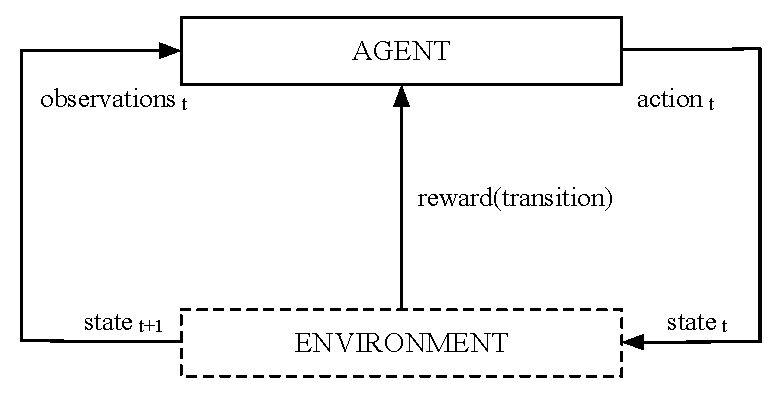
\includegraphics[width=.7\linewidth]{figures/reinforcement-learning}
  \captionof{figure}{Reinforcement Learning framework}
  \label{fig:reinforcement-learning}
\end{figure}

Figure~\ref{fig:reinforcement-learning} shows a general framework for reinforcement learning. An agent interacts with its environment in consecutive time steps. At each time step \texttt{t} the agent receives observations from the current state of the environment. It has to choose a suitable action that will cause the environment to move to a new state. A reward associated with this transition is determined and sent back to the agent.

For example, given a set of actions (such as \emph{turn-left} and \emph{turn-right}), at each step the agent applies a certain policy to its current state and to the observations it gathers from the environment to generate the next suitable action and move to the next state. While in other techniques such as supervised learning the outcome is based on historical examples and there is no concept of current state, in reinforcement learning it is all about rewards and an action resolves in a change of the state. 

% Not enough space
One of the problems in reinforcement learning is to find a policy with the right tradeoff between \emph{exploration} and \emph{exploitation}~\cite{Coggan:2004vb}. We want our agent to explore the environment and seek the best path to reach the goal and this might involve taking sub-optimal actions on the way. At the same time, we want our agent to learn from the environment and hence perform actions that are already known to be good. Finding this balance between exploration and exploitation is on of the keys to a good policy.

%\todo{explain reinforcement learning}

\section{Challenges of Reinforcement Learning}\label{sec:challenges}

% \nasser{A good paper is Hidden Technical Debt in Machine Learning Systems. D. Sculley, Gary Holt, Daniel Golovin, Eugene Davydov, Todd Phillips. in short: - Using ML erodes boundaries and diminishes encapsulation and modular design, leading to CACE principle: Changing Anything Changes Everything. This causes great difficulty to maintain the code and make isolated changes and improvements. - Unstable data dependencies are caused when input data is changing behavior over time. This can be implicit, for example, the output from an ML system that is being updated over time is used as input to another ML system. For example, consider the case in which an input signal was previously mis-calibrated. The model consuming it likely fit to these mis-calibrations, and a silent update that corrects the signal will have sudden ramifications for the model. A suggestion is to freeze the earlier models before using their output in a new ML system. - Avoid underutilized data dependencies. Examples include correlated features or features that provide little improvement. - Avoid feedback loops where, e.g., an ML system can influence its own behavior by being updated over time. - The amount of needed supporting code to use generic ML packages results in glue code system. In such conditions, trying other methods or making improvements becomes very expensive. Because a mature system might end up being (at most) 5 - The absence of good abstraction to support ML systems (similar to what exists for database technology) makes it easy to blur the lines between components. Map-Reduce is mentioned as an example of poor abstraction.  - Some hints are given on how to reduce the risks related to the configuration of ML systems. - Extra caution needed to deal with changes in external world: a simple example is when a fixed threshold value is used on the output of an ML system which is being updated over time to decide to perform an action (it’s suggested to dynamically set the threshold values in this example when applicable). Online tests and monitoring is argued to be very critical for this purpose. The main problem with ML methods is that they are optimized for average cost function and do not guarantee for corner cases. How one can verify deep learning and guarantee what is going to happen? so there is a loop: look at the verification results an improve the methods. But all is done offline, not much emphasize on online learning or self-adaptation. Big data has an important role in making this happen.}\pier{added most of it, please check the list 


%Different types of  are being used in various parts of autonomous vehicles, for example, to classify the detection of objects from sensors data. Such components 
In this section we describe some of the challenges of reinforcement learning.

\noindent {\bf Overfitting problem} - Reinforcement Learning (RL) techniques require a set of training data which have to be independent of the validation data to avoid {\em overfitting}. One main problem with machine learning methods is that they are optimized for average cost function and they do not guarantee for corner cases. Challenges in this area are comprised of the fact that when using methods such as neural networks, it is difficult for humans to understand the rules that have been learned by simply looking at its weights. This is one of the hot research areas at the moment and researchers are investigating different ways to visualize and understand the logic behind the learned neural networks in solving various tasks. Brute force testing is a widely used technique to validate the network resulting in an expensive and not always best validation method. 

\noindent {\bf Black swan} - Furthermore, because the neural network learns the rules from a training set, if certain data is missing or wrongly correlated to the training data, this can cause the network to fail and potentially cause safety hazards. In other words, if there is a special case that the system has not experienced, it cannot correctly predict such case; this is known as the {\em black sworn problem}~\cite{Nassim:2007vq}. Hence, it is hard to detect and isolate bugs where the behavior is not expressed with traditional lines of codes but entrusted to a neural network. The network would need to be retrained with also the potential risk to ``unlearn" correct behaviors. %This also motivates the safe AD architectures, where the safety of the complete system can be guaranteed.

\noindent {\bf Reward hacking} - Moreover, an incorrect specification of the reward function can cause unexpected behaviours to the agent. One of the problems is {\em reward hacking}~\cite{everitt2017reinforcement}: when the reward function is not exactly representing the designer's intention, the agent might optimize towards an imprecise reward function and behave unexpectedly. 
%meaning that the agent exploits the reward function and manages to get a high reward without achieving the designer's intentions, but instead optimizing towards the rewards function that is indeed not exactly representing the designer's intentions. 
For example, in the case of a cleaning robot, the reward function might give a positive reward for not seeing any mess then the agent might learn to disable its vision rather than cleaning up. Instead, if the reward is given only when the robot actually cleans up then the robot might learn to make a mess first and then cleaning up so that it keeps receiving more and more rewards.


%\todo{add the problem of ``avoiding side effects" and ``avoiding reward hacking" \url{\https://arxiv.org/abs/1606.06565}}

\todo{describe some of the major challenges for guaranteeing safety in autonomous vehicles as pointed out also by Koopman~\cite{Koopman:2016hh} and Schmittner~\cite{Schmittner:2014dn}.}

\todo{Add examples, like: \url{https://www.computerworld.com/article/3087328/emerging-technology/google-concerned-about-curious-but-destructive-cleaning-robots-that-hack-reward-systems.html}
\url{http://www.wired.co.uk/article/google-ai-five-problems-robots},
\url{https://blog.openai.com/concrete-ai-safety-problems/}}

%Integrating machine learning components with traditional software is a challenge that risks to lead into technical debt~\cite{Sculley:2015us}. Technical debt indicates the long-term cost that arises when implementing a quick solution that works in the short run. Besides of having all the maintainability problems of traditional software, machine learning components have special issues. Design principles, such as separation of concerns and strict abstraction boundaries, might fail to be applied in machine learning software as it uses signals from a variety of components and it has dependencies on external data. Some of the problems that the use of machine learning can cause are:

%\begin{itemize}
%    \item The use of machine learning erodes boundaries and diminishes encapsulation and modular design, leading to \emph{CACE principle}: Changing Anything Changes Everything. This causes great difficulty to maintain the code, isolate changes, and make %isolated changes and 
%    improvements. 
%    \item Unstable data dependencies are caused when input data is changing behavior over time. This can be \emph{implicit}, i.e., a machine learning system that is being updated over time; the output of such a system is used as input to another machine learning system. For example, let us consider the case in which an input signal was previously miscalibrated. The model consuming it likely fits to these miscalibrations and a silent update that corrects the signal will have sudden ramifications for the model. In order to avoid problematic situations a %A 
%    suggestion is to freeze the earlier models before using their output in a new ML system.%~\pier{TODO: rephrase maybe}
%    \item The amount of needed supporting code to use generic ML packages results in glue code system. In such conditions, trying other methods or making improvements become very expensive.
%    \item The absence of good abstraction to support ML systems (similar to what exists for database technology) makes it easy to blur the lines between components.
%    \item Extra caution needed to deal with changes in the external world: a simple example is when a fixed threshold value is used on the output of an ML system which is being updated over time to decide to perform an action (it’s suggested to dynamically set the threshold values in this example when applicable). Online tests and monitoring are argued to be very critical for this purpose. 
%\end{itemize}
    
    

%\pier{TODO: finish the sentence} %Verification of deep learning alg How one can verify deep learning and guarantee what is going to happen? so there is a loop: look at the verification results an improve the methods. But all is done offline, not much emphasize on online learning or self-adaptation. Big data has an important role in making this happen.~\pier{not clear}


			
%\section{Validation process for autonomous systems is not clear}\label{sec:approach} 

\noindent {\bf Safety assessment} - A common way to assess safety in autonomous vehicles is through extensive testing, by test-driving the vehicles, and evaluating the vehicles performance. The more the vehicles drive in autonomous mode, the more experience they gather, and this will result in % resulting in a 
continuously improving system.
Companies like Waymo\footnote{\url{https://waymo.com}} advertises that their fleet of autonomous vehicles has driven 2.5 million miles accumulating the equivalent of 400 years human driving experience. Although such numbers seem to be impressive, in order to demonstrate their reliability, autonomous vehicle might need to drive for hundreds of millions or in some cases billions of miles~\cite{Kalra:2016em}. New methods to establish the safety of autonomous vehicles are needed. Big data analysis becomes very important in this regard, statistical signal processing and machine learning methods have to be developed to analyze the large amounts of data that is collected from the test vehicles or customer vehicles. Examples of such analysis includes: (i) the detection of the use cases for which the sensors or the complete system provide poor performance, (ii) anomaly detection in the sensor data~\cite{Tashvir2017}, and (iii) the creation of realistic simulation frameworks through the use of sensor models where the logged sensor data are used to improve the quality of the %reality of the 
simulations performed in a cluster of computers. To be able to do so, sensor comparison frameworks~\cite{Florbaeck2016} are required to be able to compare the data obtained from two different sensors, where one of the sensors could have,  for example, significantly higher accuracy and can be used as a reference sensor.

Furthermore, the use of probabilistic models (as in the object detection) and stochastic algorithms (as in planning) poses new challenges in the validation process.  In fact, having %With 
probabilistic system passing the test once does not guarantee that the same test will succeed every time. %Testing becomes difficult for two reasons. The first reason is that due to the non-repeatability of such algorithms it can be difficult to exercise a particular corner case. The second reason is that it is difficult to evaluate whether a result is correct or not in the case of there are multiple correct behaviors for each test case.

\section{Controlling reinforcement learning decisions at runtime}\label{sec:approach}

In safety critical applications it is mandatory the \emph{``freedom from unacceptable risk of physical injury or of damage to the health of people, either directly, or indirectly as a result of damage to property or to the environment''}.

In this paper we present a method for delegating part of the decision-making process of an autonomous system to machine-learning, and then exploiting its flexibility and adaptability, while still preserving system's invariants. 
%However, 
%In this paper we present a method that combines the flexibility and adaptability of machine learning algorithms with the more formal and traditional invariants preservation methods.

Autonomous systems require measurements and interaction with the environment.  They perceive external information through sensors and effect the environment executing actions through actuators (in pure software system these are only inputs and outputs).  The perception of the environment is a semantic representation of the raw data and it can be achieved with techniques such as sensor fusion, where information coming from multiple sensors are combined. The perception component performs an important process that enables the autonomous system to build a model of the external world and it is the source of observations for the decision-making component.

The execution component applies the actions to the external environment and it also communicates with the internal world model. The data transferred to the world model is used to keep track of the actions generated. This information can be used for simulation purposes but also to understand the effect that actions have produced to the environment and to refine the invariants generation process.

\todo{Add simple figure describing the approach at high level}

\todo{Introduce and detail each part of the approach, identifying the challenges and how this can be realized}

\todo{discuss how the approach manages adaptation and evolution}

\subsection{Identifying invariants from high-level goals}

%\todo{get inspiration from Lammswerde and from Uchitel}
\todo{Write that we plan to exploit existing approaches and to customize them to our needs}
In our approach we need to identify invariants from important safety-critical requirements. 

Identifying from high-level goals operational requirements that should hold on components, parts of the system or operations is still an open problem. Most of the approaches that use specifications, such as formal methods, assume such operational requirements to be given. However, deriving ``correct" operational requirements from high-level goals is challenging and is often delegated to error prone processes. 

Letier and Lamwsveerde~\cite{LL02} propose an iterative approach that allows the derivation of operational requirements from high-level goals expressed in real-time linear temporal logic (RT-LTL). The approach is based on operationalisation patterns. Operationalization is a process that maps declarative property specifications to operational specifications satisfying them. The approach produces operational requirements in the form of pre-, post-, and trigger- conditions. The approach is guaranteed to be correct. Informally, here correct means that the conjunction of the operational requirements entails the RT-LTL specification. The approach is limited to a collection of goals and requirement templates provided by the authors. Moreover, the approach necessitates a fully refined goal model that requires specific expertise and is labour-intensive and error-prone.  

The tool-supported framework proposed in~\cite{AKRU99,ARRU09} combines model-checking and Inductive Logic Programming (ILP) to elaborate and refine operational requirements in the form of pre- and trigger- conditions that are correct and complete with respect to a set of system goals. System goals are in the form of LTL formulas. The approach works incrementally by refining an existing partial specification of operational requirements, which is verified with respect to the system goal. The verification is performed by using model checking, which returns a counter-example in the case of the considered property is not valid on the model. The counter-example is exploited to learn and refine the operational requirements. However, the approach
does not support learning the operational requirements for
an individual component of a system.

The work in~\cite{Bianculli2011} focuses on the service-oriented computing paradigm and starts from the observation that, when dealing with
open-world software, it is unrealistic to assume the
availability of the interface descriptions of third-party services. Then, this paper proposes an interesting approach 
to automatically generate behavioral interfaces of the partner services, by decomposing
the requirements specification of a service composition.

To avoid the wrong specification of requirements that can lead to problems similar to the reward hacking, as explained in Section~\ref{sec:challenges}, our approach plan to use user friendly ways of specifying temporal properties, such as by using structured English and specification patterns~\cite{TSE2015} or graphical languages~\cite{LSC,AIP07}.

%Authors of~\cite{CGP03} present a framework for performing assume-guarantee reasoning in an incremental and fully automatic fashion. 
%The idea to decompose the system specification into properties that should be proven valid on a system's subset, and to deduce from the local checks that the complete system satisfies the overall
%specification has been considered also by Compositional Verification. However, in general checking local properties over subsystems does not imply the correctness of the entire system. The problem is due to the existence of mutual dependencies among components. Among the several approaches proposed for compositional reasoning,  assume guarantee is one of the most promising. 
%Assume-guarantee theory has been originally introduced in the thesis of Cliff Jones~\cite{Jon81} and subsequently developed by many others, including Amir Pnueli~\cite{Pnu85}. In assume guarantee, the environment is represented as a set of properties that it should satisfy to correctly interact with the component. These properties are called assumptions, which means that they are the assumptions that a component makes on its environment. If these assumptions are satisfied by the environment, then the component that behaves in this environment will satisfy other properties, which are called guarantees. By combining the set of assume/guarantee properties in an appropriate way, it is possible to demonstrate the correctness of the entire system without constructing the complete system. 
%As testified by~\cite{CAC08}, the main difficulties of assume guarantee are (i) the assumptions generation and (ii) how to break up a system into subsystems with the purpose of efficiently verifying system properties. In this direction, the authors of
%The approach presented in~\cite{CGP03} automatically generates, via a learning algorithm, assumptions that the environment needs to satisfy for the property to hold.
%These assumptions are initially approximate, but become gradually more precise by means of counter-examples obtained by model checking the component and its environment. In~\cite{GBP05} authors observe that in reality, a component is only required to satisfy properties in certain specific environments. Moved by these motivations, they generate assumptions that exactly characterise  those environments in which the component satisfies its required property.


\subsection{Reinforcement learning for decision of autonomous systems}

In the use of reinforcement learning algorithms, two aspects are extremely important: (i) training the algorithm with the right set of data, and  (ii) specifying correctly the reward function. Referring to the first point in addition to select identify at the best we can proper training data, we support a continuous learning that involves data collected also from other systems. About the second point, 
%By embedding more domain knowledge in the reward function one could avoid the reward hacking phenomenon; this would also help the agent to learn the desired policy faster. However, as the reward functions become more complex it is harder to spot mistakes and to be confident whether the reward values that are finally sent to the agent actually reflect the designer's intentions.
we aim at providing methodologies to better engineering the reward function definition. We provide a methodology that permits to model the reward function is terms of state machines and to permit to close the gap between the designer informal goals and the reward signal. Moreover, our methodology supports the simulation and formal verification of the reward function through the use of the UPPAAL model checker\footnote{\url{http://www.uppaal.org/}}. Initial results in this direction might be found in~\cite{IRC2018}\pat{this should be anonymized}.
%of a software infrastructure that enables the verification and enforcement of reward functions to a RL agent. 



\subsection{Monitoring as controller of reinforcement learning components}

%Unlike the monitor process in the MAPE-K loop, that collects and aggregate the data from the environment, in our method the 
Runtime monitoring observes how the system is behaving and it detects if this behaviour is compliant with the system invariants. 

The main idea of runtime verification based on monitors is to synthesize a monitor that can check whether runtime behaviors satisfy or diverge from desired properties~\cite{Delgado2004,Leucker2009293}.
%Distributed and networked systems pose new challenges to monitoring with respect to monolithic systems, e.g., (i) cross-border interactions are expensive and may take place over unsafe mediums, (ii) the lack of a {\em global clock} hampers ordering of events and precise monitoring of consequentiality properties~\cite{Francalanza2013}. 
%Bauer et al.~\cite{Bauer2011} point out that two-valued semantics cannot be used to monitor all properties, such as liveness properties,
%and propose three-valued semantics called $LTL_3$. The semantics of $LTL_3$ is defined as follows: 1) satisfied; 2) violated; and 3) inconclusive. The same authors also extend $LTL_3$ with four-valued semantics: 1) satisfies the
% property, 2) violates the property, 3) will presumably violate the property, or 4) will presumably conform to the property in the future, once the system has stabilized.
Unfortunately, existing run-time monitoring approaches  provide limited information to be exploited at run-time for early detecting
and managing situations that most probably will lead to failures. 
There is the need of %We will 
investigating new approaches to automatically generate predictive monitors  
able to predict violations that most probably will happen in the near future and to provide information that can be
exploited to define strategies to prevent such failures. Our approach utilizes reinforcement learning and if the actions produced by this agent violates any safety-critical invariant the monitoring process prevents this action to be executed and \emph{tame} the agent by sending feedback. This feedback has to processed and properly expressed in term of reward function. The reinforcement learning agent will get points for its correct actions and loose points for dangerous actions that also breaks some system's invariance. 
First works in the direction of predictive monitoring might be find in~\cite{Bauer2011}, where the authors % point out that two-valued semantics cannot be used to monitor all properties, such as liveness properties,
%and 
propose three-valued semantics called $LTL_3$. The semantics of $LTL_3$ is defined as follows: 1) satisfied; 2) violated; and 3) inconclusive. The same authors also extend $LTL_3$ with four-valued semantics: 1) satisfies the
 property, 2) violates the property, 3) will presumably violate the property, or 4) will presumably conform to the property in the future, once the system has stabilized. Further research is needed to investigate approaches to automatically generate predictive monitors able to predict violations that most probably will happen in the near future and to provide information that can be exploited to define strategies to prevent such failures or to prepare suitable reactions. Monitors should offer a multi-values and fine grained semantics enabling the definition of precise
strategies to prevent possible failures. This permits the evaluation of specified properties taking into account the current status of the system and also possible evolutions of them in the near future. 

In our approach monitoring has a double purpose: 
\begin{enumerate}
    \item it \emph{monitors} the actions taken by the decision-making component preventing those that violate system's invariants from being executed. The monitor should detect the hazardous actions before they are sent to execution. For instance, referring to the automotive domain, functional safety standards such as the ISO26262 can be used as a guide for the definition of the monitored properties as in the approach of Heffernan et al.~\cite{Heffernan:2014fi}.
    \item it \emph{trains} the machine-learning algorithms by sending feedback for each produced action so that it can learn. For example, an agent that models that the behaviour of an autonomous vehicle would get a positive reward for staying in its lane, following the road, keeping a safe distance with the vehicle ahead etc. In the same way, it could loose points (hence getting a negative reward) in the case of wrong actions such as, for example, speeding or performing dangerous maneuvers. 
\end{enumerate}

 

 

 

%The goal, in this case, is to maximise the reward (or the number of points) received from the environment on which the actions are applied.

\subsection{Collecting feedback for enabling learning}

Learning is based on data that are collected from both the external environment and the internal state of the system. 
%It can be seen as the knowledge base in the MAPE-K loop, holding all the relevant information that can be used by the other components. 
Collected data are then analyzed in order to build a model of the environment that is programmatically accessible and continuously updated so that the autonomous system knows at any moment the context it is in.
%\patrizio{check this sentence}

In the case of autonomous vehicles, this component can contain a dynamic map of the world around the car and the map is continuously improved with new knowledge acquired at any time.  
%that with new knowledge being incrementally added at any time. 
%In the case of autonomous vehicles, this component can contain a symbolic representation a of dynamic map of the world around the car that is continuously updated with new data.
Currently, there are efforts in building a standardized representation of the world in the so-called ``Local Dynamic Maps"~\cite{Shimada:2015gt}. It can also contain sophisticated knowledge representations such as KnowRob~\cite{Tenorth:2015iv}, an information ontology for autonomous robots.

%An important job of this component is to set the \emph{goals} for the decision-making component. The goals are the objective to be achieved by the set of agents forming the decision-making component. This objective can be derived from the functional requirements or be specific to the type of agent in the decision-making component. For example, the goal for a reinforcement learning algorithm is to maximize the rewards obtained from the environment (represented as \emph{feedback} in the Figure~\ref{fig:loop}).

%The world model component is also responsible for sending the \emph{invariants} to be maintained to the monitoring and training component. These invariants can be generated statically from the non-functional requirements of the system. The generation of such invariants can be also dynamic hence generated from requirements that are valid only in a specific context. 
\emph{Contextual requirements} must be collected at run-time, as for instance done in Acon~\cite{Knauss:2016ce} that keeps an up to date knowledge about such context using machine learning algorithms.


\section{Conclusions}\label{sec:conclusions}

\todo{Add conclusions}

\balance

\bibliographystyle{IEEEtran}
\bibliography{library}

\end{document}